%% Basic Academic Journal Article Template
%% Author
%% John Hammersley
%% License
%% Creative Commons CC BY 4.0
%% Abstract
%% This is a basic journal article template which includes metadata
%% fields for multiple authors, affiliations and keywords.
%% It is also set up to use the lineno package for line numbers; these
%% can be turned on by adding the 'lineno' option to the documentclass
%% command.

%% Tags
%% Find More Templates
%% Basic Academic Journal Article Template
%% © 2020 OverleafPrivacy and TermsSecurityContact UsAboutBlog
%% Overleaf on TwitterOverleaf on FacebookOverleaf on LinkedIn
\documentclass[fleqn,12pt]{olplainarticle}

% Use option lineno for line numbers 

\usepackage[utf8]{inputenc}
\usepackage{graphicx}
\usepackage{hyperref}
\usepackage{microtype}
\usepackage{textcomp}
\usepackage{lineno}

\linenumbers

\title{Genotypic variation in a foundation tree results in heritable
  ecological network structure}

\author[1,2]{Matthew K. Lau}
\author[1,3,4]{Louis J. Lamit}
\author[1,5]{Rikke Reese Næsborg}
\author[6]{Stuart R. Borrett}
\author[7]{Matthew A. Bowker}
\author[1,8]{Thomas G. Whitham}

\affil[1]{Department of Biological Sciences, Northern Arizona
  University, Flagstaff, AZ 86011, USA}
\affil[2]{Harvard Forest, Harvard University, 324 N Main St,
  Petersham, MA 01366, USA}
\affil[3]{Department of Biology, Syracuse University, 107 College
  Place, Syracuse, NY 13244, USA}
\affil[4]{Department of Environmental and Forest Biology, State
  University of New York College of Environmental Science
  and Forestry, 1 Forestry Drive, Syracuse, NY 13210, USA}
\affil[5]{Santa Barbara Botanic Garden, 1212 Mission Canyon Road,
  Santa Barbara, CA 93105}
\affil[6]{Department of Biology and Marine Biology, University of
  North Carolina Wilmington, 601 South College Road, Wilmington, NC
  28403, USA}
\affil[7]{Duke Network Analysis Center, Duke University, Durham, NC
  27708, USA}
\affil[8]{School of Forestry, 200 E. Pine Knoll Dr., Northern Arizona
  University, Flagstaff, AZ 86011, USA}
\affil[9]{Center for Adaptable Western Landscapes, Northern Arizona
  University, Flagstaff, AZ 86011, USA}

\keywords{networks $|$ heritability $|$ community $|$ genetics $|$
  lichen $|$ cottonwood $|$ \textit{Populus} $|$ common garden}

%% \significancestatement{Evolution occurs in the context of ecosystems
%%   comprised of complex ecological networks. Research at the interface
%%   of ecology and evolution has primarily focused on pairwise
%%   interactions among species and have rarely included a genetic
%%   component to network structure. Here, we used a 20+ year common
%%   garden experiment to reveal the effect that genotypic variation can
%%   have on networks of lichens that colonize the bark of a foundation
%%   tree species. We found that lichen interaction network structure is
%%   genetically based and primarily driven by bark roughness. These
%%   findings demonstrate the importance of genetic variation and
%%   evolutionary dynamics in shaping ecological networks as evolved
%%   traits. In particular, this study points to the importance of
%%   assessing the effect of foundation species genetics on the structure
%%   of species interactions that can generate heritable network
%%   variation that selection can act upon.}


\begin{abstract}

%% Currently: 250 words (Thu 05 Nov 2020 10:55:40 AM EST)
  
Elucidating the genetic basis to ecological network structure is
fundamental to understanding evolution in complex ecosystems. Although
previous work has demonstrated that genetic variation can influence
food webs and trophic chains, we are unaware of a study that has
quantified the heritability of network structure of a foundation
species associated community. To examine this, in a 20+ year old
common garden we observed epiphytic lichens associated with narrowleaf
cottonwood (\textit{Populus angustifolia}), a riparian ecosystem
foundation tree species. We constructed and conducted genetic analyses
of signed, weighted, directed lichen interaction networks on
individual trees. We found three primary results. First, genotype
identity significantly predicted lichen network similarity; i.e.,
replicates of the same genotype supported more similar lichen networks
than different genotypes. Second, broad-sense heritability estimates
showed that plant genotype explained network similarity ($H^2$ =
0.41), degree ($H^2$ = 0.32) and centralization ($H^2$ = 0.33). Third,
of several tree phenotypic traits examined, bark roughness was both
heritable ($H^2$ = 0.32) and significantly predicted lichen network
similarity ($R^2$ = 0.26). These results support a mechanistic,
genetic pathway from variation in a heritable tree trait to ecological
network structure and demonstrate that evolution has the potential to
act at the community level to influence not only abundances of
organisms but also interactions at the scale of entire networks.

\end{abstract}

\begin{document}

\flushbottom
\maketitle
\date
\thispagestyle{empty}

\section*{Introduction}

Evolution occurs in the context of complex ecological
networks. Community genetics studies have shown that genetic variation
in foundation species, which have large effects on ecosystems by
modulating and stabilizing local conditions \citep{Ellison2005}, plays
a significant role in defining distinct communities of interacting
organisms: such as endophytes, pathogens, lichens, arthropods, and
soil microbes \citep{Busby2015, Barbour2009c, Lamit2015c}. Multiple
studies have now demonstrated that genetic variation influences
numerous functional traits (e.g., phytochemical, phenological,
morphological) that in combination result in a multivariate functional
trait phenotype \citep{Holeski2012} in which individual plant
genotypes support different communities and ecosystem processes
\citep{Bailey2009a, Whitham2012afix}. Recently, the importance of genetic
variation in structuring ecological systems was reviewed, and not only
were many instances of strong genetic effects found in many ecosystems
but the effect of intraspecific variation was at times greater than
inter-specific variation \citep{DesRoches2018TheVariation}. There is
now evidence to support that selection occurs among groups of species
\citep{Wade2007TheCommunities} and that genetic variation and
phylogenetic relatedness contribute to variation in community assembly
\citep{Crutsinger2016} and species interactions \citep{Whitham2006a,
  Bailey2009a, Moya-Larano2011}. These evolutionary dynamics have the
potential to shape the structure of ecological interaction networks
\citep{Rezende2007, Guimaraes2007InteractionNetworks,
  Gomez2009LocalMosaic}.

Empirical and theoretical work in network ecology and evolutionary
biology point to the need for examinations of the genetic basis of
ecological network structure. Analyses of ecological networks have
demonstrated that indirect effects can lead to self-organization,
producing sign-changing, amplifying and/or dampening effects
\citep{Fath1998, Newman2006, Sole2006Self-OrganizationEcosystems} and
other studies have demonstrated that indirect effects of interactions
among species can lead to network structures that amplify or dampen
the effects of selection, such as the formation of star-like
structures in which there is a ``central'' species or core group of
species \citep{Lieberman2005EvolutionaryGraphs}. Also, work by
\cite{Toju2014a, Toju2016, Toju2017} observed consistent patterns of
centralized interactions of species modules (i.e., groups of species
that interact more strongly within their group than with other
species) focused around hubs of plant-fungal interactions. In other
words, a small number of plant and fungal symbionts tended to have
disproportionate numbers of interactions with other species and likely
are the drivers in determining community assembly, structure and
dynamics.  Interspecific indirect genetic effects (IIGE) theory
(\textit{sensu} \cite{Shuster2006COMMUNITYSTRUCTURE-fix}) in evolutionary
biology also points to the importance of studying the genetics of
interaction network structure. Genetically based differences in
network structure among individuals can be acted upon by natural
selection when there are fitness consequences of different networks of
IIGEs, leading to community evolution per
\cite{Whitham2020IntraspecificEvolution} and, by extension,
interaction network evolution. For example, although the analysis was
of abundances rather than interaction networks,
\cite{Gehring2014PlantChange, Gehring2017afix} found that the mycorrhizal
communities on the roots of drought tolerant and intolerant trees are
dominated by different orders of ectomycorrhizal fungal mutualists
that also differ in the benefits they provide that enhance tree
performance. Because drought tolerant genotypes are three times more
likely to survive record droughts, selection acts both on the tree and
its fungal community and with increased drought the community
phenotype has changed over time. Also, in an antagonistic interaction
context, \cite{Busby2015} found that with the addition of a damaging
leaf pathogen to cottonwoods in a common garden, the impacts of these
strong interactors results in a different and diminished community of
arthropods relative to control trees. These examples collectively
support the possibility that selection acting on the tree may alter
the network structure of associated communities in which different
networks are more likely to survive drought and pathogen outbreaks,
respectively. Regardless of whether the IIGE is unilateral (i.e., tree
affects the community) or reciprocal (i.e., the community also affects
the relative fitness of the tree), selection at the level of the tree
population or its community, or both, can change network structure and
alter community dynamics \citep{Whitham2020IntraspecificEvolution}.

In this context, the ``genetic similarity rule'' of community genetics
provides a useful framework we can apply to interaction networks at
the nexus of ecological and evolutionary dynamics. In a study
combining experimental common gardens and landscape-scale observations
of interactions between \textit{Populus} spp.  (cottonwoods) and
arthropods, \cite{Bangert2006} observed that individual genotypes that
are more genetically similar will tend to have similar phytochemical
traits and thus tend to have similar interactions with other
species. Although this is likely to have consequences for interactions
and network structure, studies in the network ecology literature
generally do not include a genetic component \citep{Lau2017a} and
community genetics studies have primarily focused on community
composition in terms of the abundance of species
\citep{DesRoches2018TheVariation}. Some studies have examined the
effects of genetic variation on trophic chains in plant-associated
communities (including \textit{Populus}, \textit{Solidago},
\textit{Oenothera}, \textit{Salix})
\citep{Bailey2006fix, Johnson2008, Smith2011,
  Smith2015b, Barbour2016GeneticComplexity} and generally found that
increasing genotypic diversity leads to increased trophic
complexity. We are aware of only two studies that explicitly examined
the effect of genotypic variation on interaction networks between tree
individuals and associated herbivores using ecological network metrics
\citep{Lau2016afix, Keith2017}. Both found that genotypic diversity
generates increased network modularity (i.e., compartmentalization);
however, both were examining networks at the scale of forest stands,
rather than networks associated with individual trees; therefore,
neither was able to observe replicated networks in order to
statistically test for genetic effects on network structure and
quantify the genetic component (i.e., heritable variation) in network
structure.

Here, we investigate how genetic variation in a foundation tree
species determines the structure of a network of interactions among a
community of tree associated lichens.  We used a long-term (20+
years), common garden experiment with clonally replicated
\textit{Populus angustifolia} individuals of known genetic identity
\citep{Martinsen2001HybridSpecies}. We focused on a community of
epiphytic lichen species, as previous research has demonstrated
significant compositional effects of genotypic variation on lichen in
this system \citep{Lamit2011, Lamit2015a, Lamit2015c} and epiphytic
organisms in other systems \citep{Winfree2011, Zytynska2011}. Applying
a probability-theory based network modeling approach
\citep{Araujo2011}, we constructed a set of interaction network models
for the lichens associated with individual trees. Using these models,
we then examined the genetic basis of the structure of these
ecological networks via several network metrics that measure different
aspects of network structure at the scale of individual species (i.e.,
nodes) or the entire network observed on each tree genotype. Given the
potential importance of focal or ``central'' nodes (e.g., species) for
determining network dynamics \citep{Lieberman2005EvolutionaryGraphs},
we focused on network metrics that measure centrality for individual
species and centralization for whole networks. Both of these metrics
measure how much a species is connected in the network relative to
other species. As there is a preponderance of evidence that in natural
systems evolution occurs in communities comprised of networks of
interacting species \citep{Lau2016afix, Keith2017, Thompson2013,
  Bascompte2006}, we set out to test two hypotheses. First, per the
genetic similarity rule \citep{Bangert2006} and IIGE theory
\citep{Whitham2020IntraspecificEvolution}, we hypothesize that trees
of the same genotype (i.e., clones) will support more similar lichen
interaction networks relative to individuals of other genotypes. In
other words, epiphytic lichen network structure is heritable, which
can be calculated via comparisons of within and among group variation
in network structure. Second, heritability of lichen network structure
is the result of underlying phenotypic covariation in tree traits
important to interactions between trees and lichens and among
lichens. Evidence that such trait covariance generates variation in
interactions among community members provides an intermediate
genetics-based mechanism for the underlying factors determining lichen
distribution and abundance. In combination, evaluating these two
hypotheses is fundamental to understanding variation and dynamics of
network structure and evolution.


\section*{Materials and Methods}


\subsection*{Study System}

The study was conducted along the Weber River, UT (USA), which is a
cottonwood (\textit{Populus} spp.) dominated riparian
ecosystem. Although two native species, \textit{Populus angustifolia}
(James) and \textit{Populus fremontii} (S. Watson), occur here and are
known to hybridize, in order to focus on intra-specific genetic
variation we only sampled pure or advanced generation back-crosses of
\textit{P. angustifolia}. Bark lichens have been
intensively sampled in this system and provide an ideal community in
which to observe and model interaction networks, as their sessile
nature permits accurate identification of individuals and their highly
localized, direct contact interactions and slow population turnover
rates facilitate the assessment of interactions among lichen species
on individual trees \citep{Lamit2015a}.

A long-term, common garden experiment was used to isolate the effect
of tree genotype from the effect of the localized microenvironment
associated with each individual and spatial
autocorrelation. Established in 1992, asexually propagated clones of
genotyped \textit{P. angustifolia} individuals were obtained from wild
collections and planted in a fully randomized design at the Ogden
Nature Center, Ogden, UT. From the population of established
individuals in the common garden, we sampled a total of ten genotypes,
replicated between 3 and 8 times each. These individuals comprised a
set of tree genotypes with lichen communities that have been well
studied by previous investigations \citep{Lamit2011,
  Lamit2015a, Lamit2015c}.



\subsection*{Bark Lichens and Trait Observations}


We conducted a modified sampling procedure originally developed by
\cite{Lamit2015a}. On each tree, presence or absence of each lichen
species was assessed in a total of 50 1 cm$^2$ cells arrayed in a 10
cm$^2$ checkerboard pattern. Given the small size and sessile nature
of lichens, we were able to rapidly assess lichen interactions by
quantifying thalli of different species occurring in close
proximity. Sampling was restricted to the northern aspect of the trunk
to maximize the abundance of lichens and control for the effect of
trunk aspect. Two adjacent 100 cm$^2$ quadrats centered at 50 cm and
95 cm from ground level were sampled
(Fig~\ref{fig:lichen_sampling}). The observed lichen community
included: \textit{Athallia holocarpa}, \textit{Candelariella
  subdeflexa}, \textit{Myriolecis hagenii}, \textit{Rinodina freyi},
\textit{Physcia adscendens}, \textit{Physciella melanchra},
\textit{Physcia undulata}, \textit{Xanthomendoza galericulata},
\textit{Xanthomendoza montana}. Several other species were not
observed in the present study but are known to occur in this region:
\textit{Melanohalea elegantula}, \textit{Melanohalea subolivacea},
\textit{Phaeophyscia ciliata} and \textit{Phaeophyscia orbicularis}.

The cell size and checkerboard sampling pattern was chosen to isolate
the individuals in each cell. In a survey of \textit{Xanthomendoza
  galericulata} in the common garden, we had observed a median thallus
size of 0.12 $\pm$ 0.001 cm$^2$ (1 S.E.)  (Supporting Information,
Fig. 1). This expected thallus size formed the basis for our sampling
design, such that lichen observations were spatially independent of
thalli present in other cells but exposed to similar
micro-environmental conditions created by the bark and the location of
the sampling area on an individual tree. Therefore, we were confident
in treating the cell-wise observations in quadrats as independent with
respect to lichen-lichen interactions. 

We quantified tree traits inside or in close proximity to the lichen
quadrats. Selected traits have been demonstrated previously to be
under strong genetic control in cottonwoods \citep{Bdeir2017} and
other foundation tree species, such as \textit{Eucalyptus}
\citep{Nantongo2020}, and previous work has provided evidence for
effects on lichen communities of some of these traits
\citep{Lamit2011}. We assessed bark texture/structure, hereafter
referred to as roughness, in the quadrat as the percent of 1 cm$^2$
cells with ``rough'' bark, i.e., bark containing a fractured
surface. In addition, we also examined several bark chemistry traits
by taking bark samples immediately adjacent to each quadrat. We used
previously collected phytochemical data from \cite{Lamit2011},
including the concentration of condensed tannins, carbon and
nitrogen. Additionally, we quantified bark pH for each tree.  Bark
samples were collected by excavating adjacent to the quadrat down to a
depth of 2 mm. Bark pieces were air dried for storage and later
processing. Samples were prepped for pH measurements by crushing with
a mortar and pestle until all pieces were approximately 0.5 cm in
diameter, creating equivalent surface areas among samples. 0.5 g of
crushed bark was placed in a 15 ml Falcon collection tube with 5 ml of
deionized water. Tubes were capped and let sit for 24 hrs prior to pH
measurement with a SevenGo\texttrademark\ pH meter (Mettler Toledo).


\begin{figure}[ht]
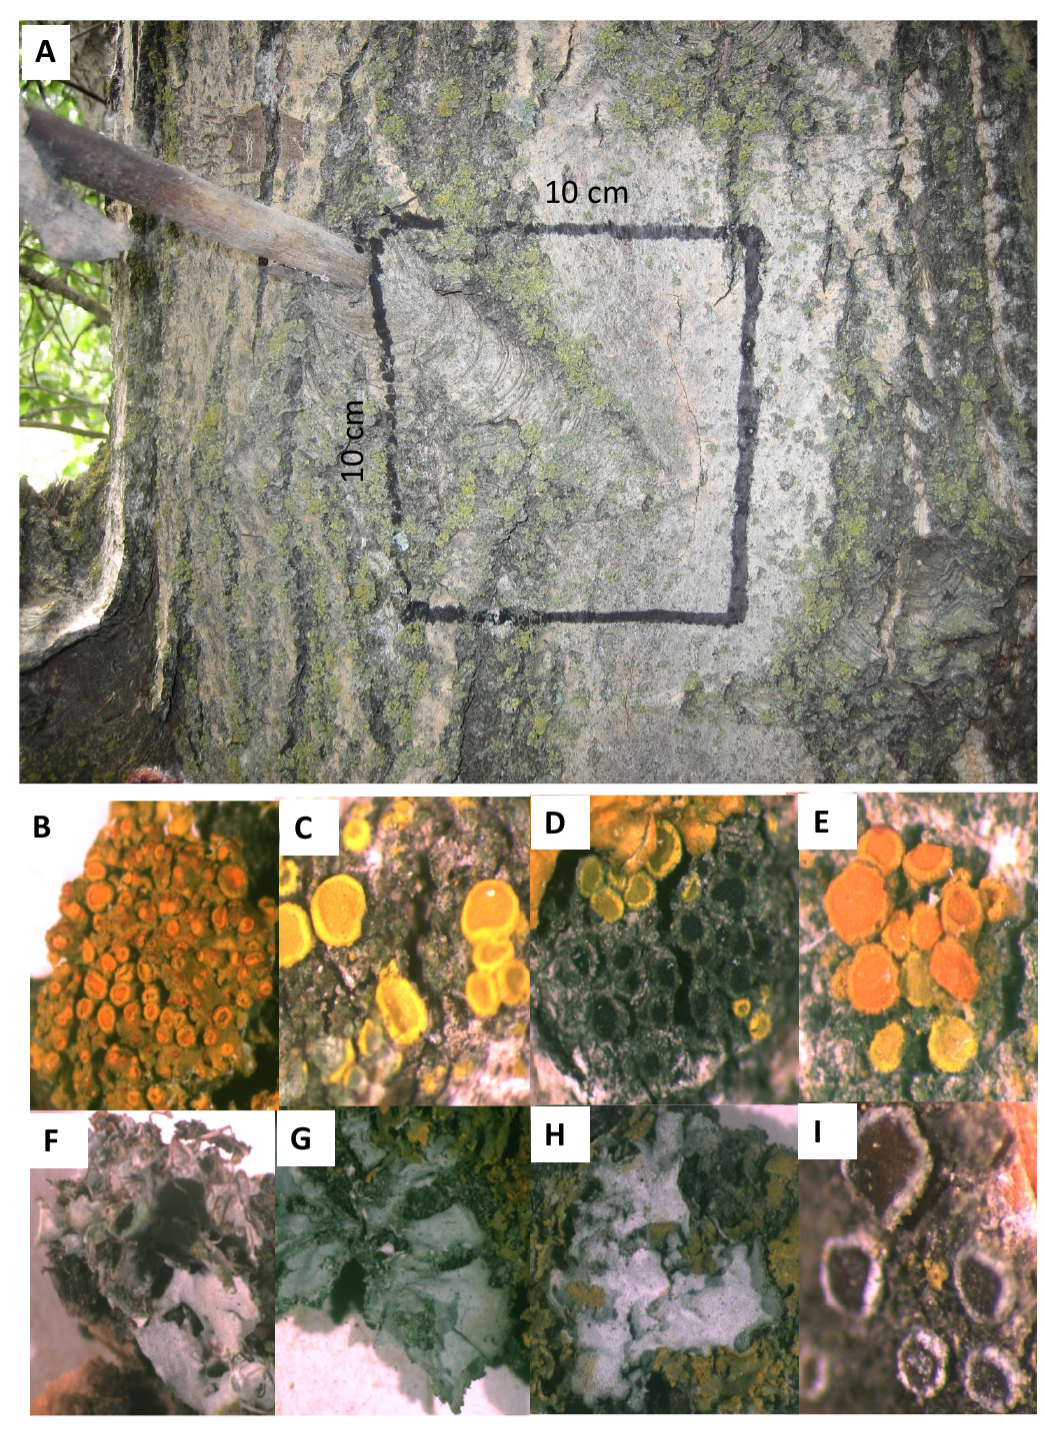
\includegraphics[width=0.90\linewidth]{figures/lcn_sampling.png}
\caption{The communities of bark lichens were observed in a common
  garden of replicated genotypes of narrowleaf cottonwood trees
  (\textit{P. angustifolia}) at the Ogden Nature Center (Ogden,
  UT). (A) Lichens were sampled within a fixed area (100 cm$^2$) on
  individual trees at two heights, 50cm and 95cm from the
  ground. (B-I) Photos showing lichen species observed, respectively:
  \textit{Xanthomendoza montana}, \textit{Candelariella subdeflexa},
  \textit{Rinodina freyi}, \textit{Athallia holocarpa},
  \textit{Physcia adscendens}, \textit{Physciella melanchra},
  \textit{Physcia undulata} and \textit{Myriolecis hagenii}. Photo
  Credits: L.J. Lamit (B-D) and R. Reese Næsborg (E-I).}
\label{fig:lichen_sampling}
\end{figure}


\subsection*{Lichen Network Modeling}

For each tree, the repeated observations of lichens were used to
construct replicated interaction networks, i.e. one for each
individual tree. Unipartite networks were generated using the
conditional probabilities of each species pair, i.e., the probability
of observing one species given an observation of another species
$P(S_i | S_j)$, based on the method developed by \cite{Araujo2011}. To
calculate conditional probabilities, we quantified the individual
probabilities of species occurrences $P(S_i)$ and the joint
probability of co-occurrences $P(S_i, S_j)$ using the frequencies of
each species and their co-occurrences. Using the axioms of
probability, we can calculate the conditional probabilities of each
species pair as $P(S_i|S_j) = \frac{P(S_i,S_j)}{P(S_j)}$. This yields
a matrix that could possibly be asymmetrical, i.e., $P(S_i|S_j)$ does
not have to be equal to $P(S_j|S_i)$. Also, the diagonal, $P(S_{i} |
S_{i})$, is equal to one for all species present and zero for species
that were not observed in any cell.

We then applied an analytical procedure to remove non-significant
links between species. This procedure determines if the joint
probability of a species pair (i.e., $P(S_i,S_j)$) is different from
zero (Fig.~\ref{fig:conet_method}).  Here, a confidence interval
$CI_{95\%}$ is calculated as as $CI_{95\%} = E[S_iS_j] * Z_{95\%} *
\sqrt{V(S_iS_j)}$, where the expected frequency of co-occurrences
E($S_iS_j$) is the total number of cells surveyed ($N$) times the
independent probabilities of each species $P(S_i) * P(S_j)$,
$Z_{95\%}$ is the Z-score for 95\% from a Z-distribution and the
expected variance of $E(S_iS_j)$ is the total number of cells times
the expected probability of $S_iS_j$ and its compliment (i.e.,
$V(S_iS_j) = N * E[P(S_i,S_j)] * (1 - E[P(S_i,S_j)])$). If the
observed number of co-occurrence falls within the confidence interval,
the joint probability $P(S_i,S_j)$ is concluded to be equal to the
product of the individual probabilities (i.e., $P(S_i) \dot P(S_j)$),
and the conditional probability reduces to the individual probability
of that species $P(S_i)$. Therefore, unless the co-occurrence of a
species pair falls outside the confidence interval, the probability
that the observation of one species given the other is no different
than simply observing that species alone. This enables us to remove
links from a given network by re-scaling the resulting conditional
probabilities through subtraction of the individual probabilities from
the conditional probabilities (i.e., how different the conditional
probability is from the independent probability), which makes any
species with a non-significant conditional probability zero.

The resulting matrix ($\mathbf{D} = D_{ij}$) can be interpreted as one
species' impact on another with zero being no effect and values less
than or greater than zero being negative and positive effects,
respectively. We will refer to $\mathbf{D}$ as a signed, weighted
interaction matrix. As such, $\mathbf{D}$ has the properties that it
can be asymmetric (i.e., $D_{ij}$ does not necessarily equal $D_{ji}$)
and that it scales between -1 and 1, and, therefore, does not have the
mathematical properties of a probabilistic network
\citep{Poisot2016TheNetworks}. Also, as the method does not track
individuals within species; therefore, the ``intra-specific''
observations are the same species being counted across the cells of
the grid and a resulting $D_{ii} = 0$. In the context of these
networks, asymmetry and positive/negative valued connections are
distinct quantities. In-coming and out-going connections can be
interpreted as ``influenced by'' and ``influenced'', respectively;
while positive and negative are within this study interpreted as one
species increasing or decreasing, respectively, the probability of
another species' occurrence.

\begin{figure*}[ht]
\centering
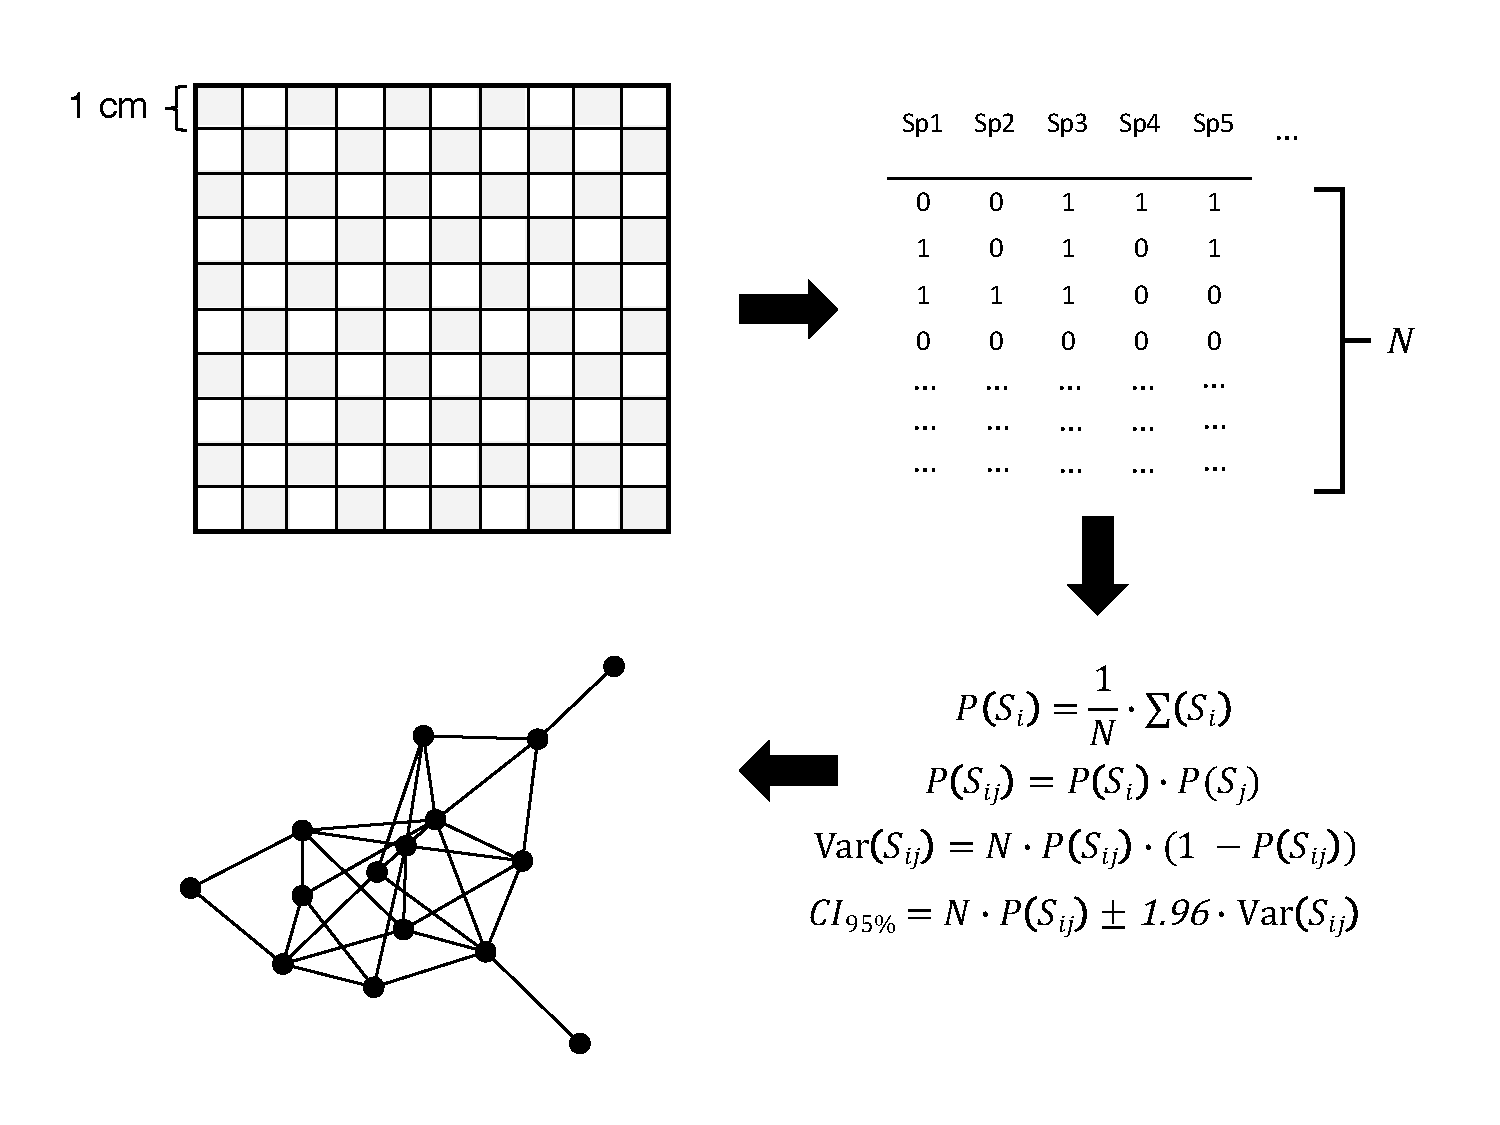
\includegraphics[width=\linewidth]{figures/lcn_araujo_method.pdf}
\caption{Lichen interaction networks were constructed by conducting
  field observations in 1 cm$^2$ cells within a 100 cm$^2$ grid on each
  tree using a checkerboard pattern (grey cells). Thus, a set of $N$
  total cell observations were recorded for each tree with the
  presence or absence of each species recorded for each cell. Applying
  the probability-based network modeling method adapted from
  \citep{Araujo2011}, we calculated the conditional probabilities,
  $P(S_i|S_j)$, for all species pairs and removed (i.e., set equal to
  zero) species pairs whose joint probabilities, $P(S_i S_j)$, were
  not significant using a confidence interval based comparison of
  their observed co-occurrence frequency, $S_iS_j$, to that expected
  due to chance alone, $E[P(S_iS_j)] = P(S_i) P(S_j)$, and
  $P(S_i|S_j)$ reduces to $P(S_i)$, the observed individual
  probability of species $S_i$.}
\label{fig:conet_method}
\end{figure*}


\subsection*{Analyses, Software and Data}

To quantify the structural variation of lichen networks we calculated
several metrics at both the level of node and whole networks. Although
there are many other network metrics, for the sake of simplicity we
focus on a subset that represent the primary interesting features of
network structure, see \cite{Lau2017a}. We calculated the number of
interactions or ``links'' in each network (degree), which provides a
measure of the size of the network \citep{Lau2016afix,
  Borrett2014EnaR:Analysis}. We also calculated the centralization of
each network using Freeman's centrality, which measures the evenness
of the distribution of interactions among the species in the network,
using the \texttt{sna} package \citep{sna}. In a network with low
centralization species have similar strengths and numbers of
interactions. A network with high centralization tends to have one or
a small number of species that interact with other species. We used a
related function to calculate the centrality of each species (i.e.,
node level centrality) in each network as well. To calculate separate
metrics for positive and negative links, as the networks contained not
only positive and negative connections but also directional
connections (both in-coming and out-going), we calculated the same
network metrics for all combinations of these types of connections
using recently developed methods for signed, weighted and directed
networks \citep{Everett2014NetworksTies} using the \texttt{signnet}
package \citep{signnet}.

We used a combination of parametric and non-parametric, permutation
based frequentist statistical analyses to test for the effects of
genetic variation on lichen communities and their interaction
networks. To assess the effect of genotype on traits as univariate
response variables (including the metrics of network structure), we
used additive, random effects models with Restricted Maximum
Likelihood (REML) conducted in R via the \texttt{lme4} and
\texttt{RLRsim} packages \citep{lme4, RLRsim}. To conform to test
assumptions, traits were root transformed with the exception of
condensed tannin concentration and carbon-nitrogen ratio, which were
rank and log$_{10}$ transformed, respectively. Differences in node
level centrality among species was tested using ANOVA and Tukey-HSD
multiple comparison tests. Correlations among trait variables and
network metrics were quantified and tested using linear correlations
of Pearson's $r$. For multivariate response variables, such as lichen
community composition and network structure, we used distance based
multivariate statistical approaches. To quantify the similarity of
lichen networks among individual trees, we calculated the pairwise
Euclidean distance of the $\mathbf{D}$ interaction matrices among all
trees \citep{Newman2010}. For community composition we applied
Bray-Curtis similarity to a matrix of species abundances obtained by
aggregating the gridded observations by summing over the binary
cell-wise species presence-absences. To test for the effects of
genotype and other predictor variables on community and network
similarity we conducted Permutational Analysis of Variance (PERMANOVA)
with \texttt{vegan} \citep{vegan} using 100000 permutations. For
visualization of multivariate patterns, we used Non-metric
Multi-Dimensional Scaling (NMDS) \citep{ecodist} to produce
dimensionally reduced ordinations of these multivariate responses and
fitted vectors for continuous predictor variables to the ordinated
values \citep{vegan}, using 100 random initial configurations with a
maximum of 1000 iterations and a change in stress threshold of less
than 10$^{-12}$. This was repeated for one to four dimension
configurations, and the configuration with the lowest dimensionality
and an unexplained variation less than 10\% was selected. For all
tests where genotype was used as a predictor, we quantified the
heritability of the response variable. Because the trees in the garden
were clonal replicates of each genotype, we calculated broad-sense
heritability, which is the genotypic variance divided by the total
phenotypic variance \citep{Conner2004ATextbook}, which can be
interpreted as a measure of the phenotypic variance due to genotypic
variation. All analyses were conducted using R version 4.0.2
\citep{R2020}. Code and data for the project are openly available as a
reproducible workflow using \texttt{drake} \citep{drake} archived via
Zenodo \url{https://doi.org/10.5281/zenodo.4581639}.

\begin{figure}[ht]
\centering
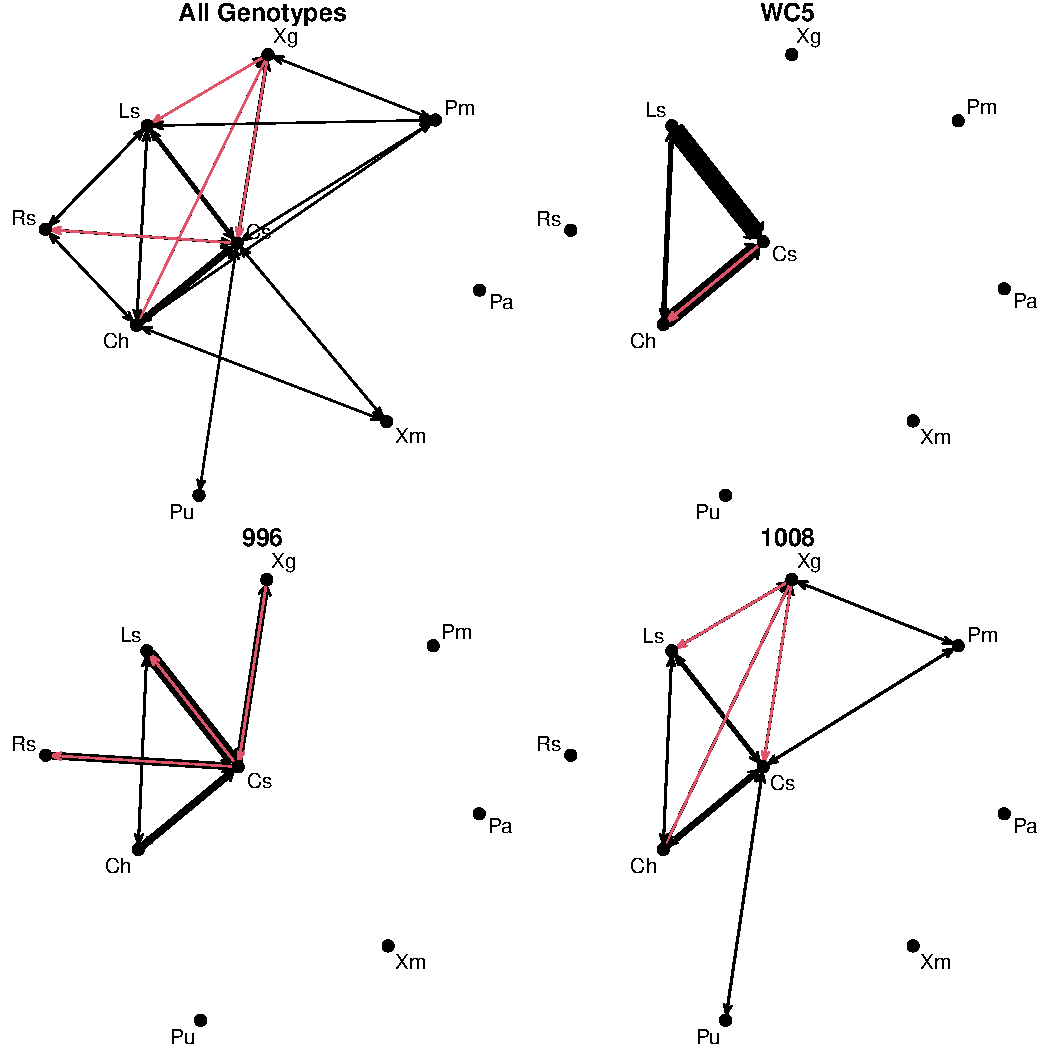
\includegraphics[width=\linewidth]{figures/cn_onc.pdf}
\caption{Lichen networks varied in structure among tree
  genotypes. Network diagrams of the mean lichen interaction matrices
  averaged for all trees and for illustrative genotypes (996, WC5 and
  1008) showing a range of interaction network
  structure. Directionality (arrowheads) and sign (red = negative,
  black = positive) of interactions are shown as edges between
  species, which are scaled by their magnitude.  Species names are
  abbreviated by the first letter of the genus and specific epithet:
  Ah = \textit{Athallia holocarpa}, Cs = \textit{Candelariella
    subdeflexa}, Mh = \textit{Myriolecis hagenii}, Rf =
  \textit{Rinodina freyi}, Pa = \textit{Physcia adscendens}, Pm =
  \textit{Physciella melanchra}, Pu = \textit{Physcia undulata}, Xg =
  \textit{Xanthomendoza galericulata}, Xm = \textit{Xanthomendoza
    montana}. The sign of the interaction is indicative of greater
  (positive) or lesser (negative) paired occurrences than expected
  relative to the overall frequency of occurrence of each
  species. Ecologically, the links in the network are likely the
  product of multiple types of interactions (e.g. mutualism,
  parasitism, competition, facilitation) that could vary over both
  space and time.}
\label{fig:geno_nets}
\end{figure}

\section*{Results}

In support of our first hypotheses, we found that tree genotype
influenced lichen network structure and that multiple lichen network
metrics were heritable. Tree genotype significantly predicted the
structural similarity of lichen networks and, overall, network-level
metrics responded significantly to tree genotype, including network
degree and centralization including both in-coming and out-going links
or when separated into in-coming only or out-going only
(Table~\ref{tab:h2_net}, Fig.~\ref{fig:h2_plot}).  Metrics including
only positive links also showed a significant effect of tree genotype,
including positive degree and positive in-going centralization.
Metrics calculated with negative links were not significant, including
degree (negative) and both in-coming (negative) and out-going
centralization (negative). Interestingly, although network similarity
and multiple network metrics were significantly predicted by tree
genotype, we did not observe a significant genotypic effect for
community composition (Pseudo-$F_{9, 27}$ = 0.751, R$^2$ = 0.20,
\textit{p-value} = 0.888).

\begin{figure*}[ht]
\centering
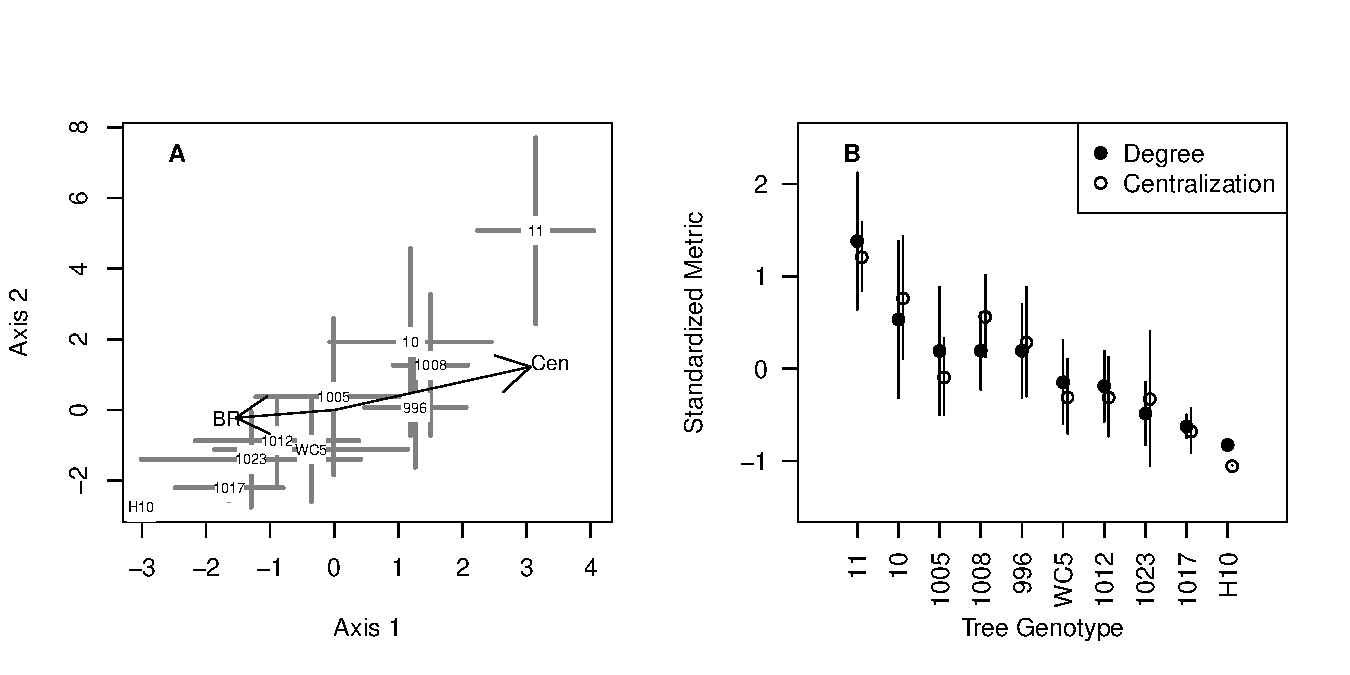
\includegraphics[width=\linewidth]{figures/h2_plot.pdf}
\caption{The similarity of lichen networks varied among tree
  genotypes. A. The plot shows genotype centroids of NMDS ordinated
  (R$^2$ = 0.999, stress = 0.008) lichen network similarity ($\pm$ 1
  S.E.). Genotype centroids that are closer together tend to have more
  similar lichen network structure. Arrows showing the direction
  (arrowhead) and magnitude (length) of the vectors of correlation
  between bark roughness (\textbf{BR}) and network centralization
  (\textbf{Cen}) and the ordinated networks. B. Plot showing
  the standardized ($\frac{x - \bar{x}}{\sigma}$) means ($\pm$ 1 S.E.)
  for the two of the genetically based lichen network metrics: overall
  degree (i.e., total number of links) and centralization, which is a
  measure of the dominance of one species in the network.}
\label{fig:h2_plot}
\end{figure*}

% latex table generated in R 3.6.3 by xtable 1.8-4 package
% Wed Dec  2 18:23:39 2020
\begin{table}[ht]
\centering
\begin{tabular}{rrrrr}
  \hline
Response & df & $RLRT$ & $H^2$ & p-value \\ 
  \hline
Lichen Network Similarity & 9 & 3.5821 & 0.41 & 0.0537 \\ 
  Degree & 9 & 3.5175 & 0.32 & 0.0255 \\ 
  Degree (positive) & 9 & 3.6925 & 0.32 & 0.0229 \\ 
  Degree (negative) & 9 & 0.0327 & 0.03 & 0.3859 \\ 
  Centralization & 9 & 4.0444 & 0.33 & 0.0184 \\ 
  Centralization In-Degree & 9 & 4.4812 & 0.35 & 0.0142 \\ 
  Centralization In-Degree (positive) & 9 & 3.9852 & 0.33 & 0.0190 \\ 
  Centralization In-Degree (negative) & 9 & 0.3304 & 0.11 & 0.2508 \\ 
  Centralization Out-Degree & 9 & 3.8615 & 0.32 & 0.0205 \\ 
  Centralization Out-Degree (positive) & 9 & 3.5585 & 0.31 & 0.0248 \\ 
  Centralization Out-Degree (negative) & 9 & 0.0862 & 0.05 & 0.3446 \\ 
   \hline
\end{tabular}
\caption{Genotypic effects on the associated lichen network structure. $RLRT$ is the statistic from the restricted likelihood ratio tests.} 
\label{tab:h2_net}
\end{table}


The genetic response of network centralization was driven by variation
in \textit{Athallia holocarpa}. Centrality varied significantly among
species ($F_{8, 324}$ = 7.99, $R^2$ = 0.16, \textit{p-value} $<$
0.0001). The node-level metrics for \textit{A. holocarpa} displayed
the strongest response to tree genotype with high levels of
heritability of positive centrality for both the in-coming
(\textit{RLRT} = 3.61, $H^2$ = 0.32, \textit{p-value} = 0.0240) and
out-going (\textit{RLRT} = 3.13, $H^2$ = 0.30, \textit{p-value} =
0.0327) perspectives but not for either negative centrality metrics
in-coming (\textit{RLRT} = 0, $H^2$ = 0, \textit{p-value} = 1) or
out-going (\textit{RLRT} = 0, $H^2$ = 0, \textit{p-value} =
0.4543). None of the other species' centralities showed a genotypic
response (Supporting Information, Fig. 2) with the exception of
\textit{X. montana} (\textit{RLRT} = 2.92, $H^2$ = 0.32,
\textit{p-value} = 0.0375); however, the centrality of
\textit{X. montana} was much lower overall relative to
\textit{A. holocarpa} and the variation in \textit{X. montana}
centrality was restricted to two genotypes
(Fig.~\ref{fig:geno_sppcen}).



\begin{figure*}[ht]
\centering
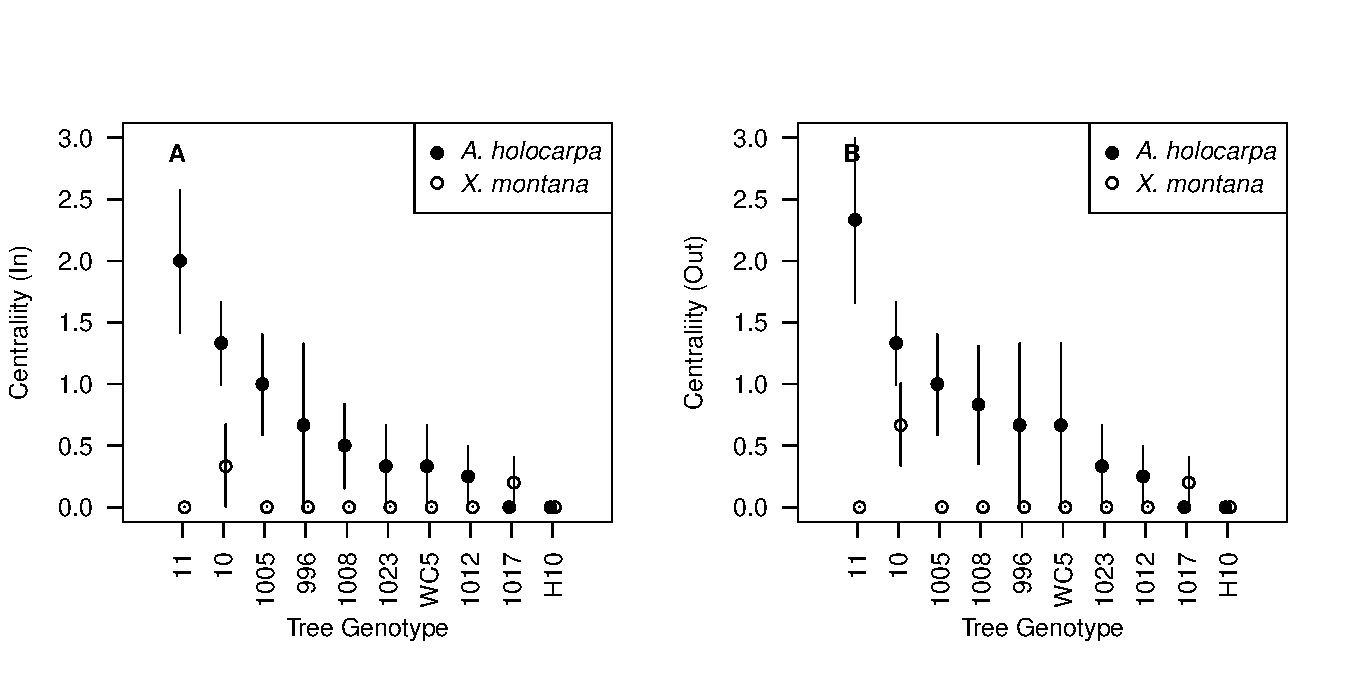
\includegraphics[width=\linewidth]{figures/geno_sppcen.pdf}
\caption{Dot-plots showing the mean (dot) and $\pm$ 1 SE of in-degree
  (A) and out-degree (B) centrality for two species,
  \textit{A. holocarpa} and \textit{X. montana}. \textit{Athallia
    holocarpa} centrality was highly variable among
  genotypes. \textit{Xanthomendoza montana} centrality, both in- and
  out-degree, was only non-zero for two genotypes, and only out-degree
  centrality displayed a significant response to genotype.}
\label{fig:geno_sppcen}
\end{figure*}

In support of our second hypothesis, analysis of trait covariation
revealed that genotype indirectly influenced lichen network
centralization via genetically based variation in bark roughness. The
percent cover of rough bark (\textit{RLRT} = 4.8526, $H^2$ = 0.3221,
\textit{p-value} = 0.0113) and condensed tannins (\textit{RLRT} =
3.0522, $H^2$ = 0.3205, \textit{p-value} = 0.0343) both displayed
significant responses to tree genotype. None of the other bark traits,
pH (\textit{RLRT} = 0.00, $H^2$ = 0.00, \textit{p-value} = 1.0000) or
carbon-nitrogen ratio (\textit{RLRT} = 0.0000, $H^2$ = 0.0000,
\textit{p-value} = 1.0000), showed a significant response to tree
genotype and none other than bark roughness was correlated with
network similarity (Table~\ref{tab:cn_trait_perm}); therefore, we
focused our subsequent analyses on the indirect effect of genotype on
lichen network structure via bark roughness. We found that bark
roughness was significantly correlated with network similarity and
other lichen network metrics, including negative correlations with
overall network degree ($df$ = 35, $t$ = -2.13, $r$ = -0.34,
\textit{p-value} = 0.04) and centralization ($df$ = 35, $t$ = -2.52,
$r$ = -0.39, \textit{p-value} = 0.02). In other words, trees with more
similar levels of bark roughness tended to have lichen interaction
networks with similar structure (Fig.~\ref{fig:br_net}). To quantify
the genetic bases of this effect of bark roughness on network
structure, we used the residual values from regressions of the network
metrics and bark roughness in subsequent tests of the effect of tree
genotype and found no significant effect of tree genotype for either
degree (\textit{RLRT} = 0.00, $H^2$ = 0.00, \textit{p-value} = 1.0000)
or centralization (\textit{RLRT} = 0.00, $H^2$ = 0.00,
\textit{p-value} = 1.0000), and, thus, the bulk of the genetically
based variation in the network metrics can be explained by bark
roughness.

% latex table generated in R 4.0.2 by xtable 1.8-4 package
% Mon Feb  1 17:29:25 2021
\begin{table}[ht]
\centering
\begin{tabular}{rrrrrr}
  \hline
 & df & SS & R2 & Pseudo-F & p-value \\ 
  \hline
Bark Roughness & 1 & 20850.09 & 0.26 & 12.9234 & 0.0101 \\ 
  Condensed Tannins & 1 & 5993.66 & 0.07 & 3.7150 & 0.0813 \\ 
  pH & 1 & 1273.19 & 0.02 & 0.7892 & 0.3712 \\ 
  Carbon:Nitrogen Ratio & 1 & 3896.18 & 0.05 & 2.4150 & 0.1890 \\ 
  Residual & 32 & 51627.33 & 0.64 &  &  \\ 
  Total & 36 & 80993.59 & 1.00 &  &  \\ 
   \hline
\end{tabular}
\caption{PERMANOVA Pseudo-F Table of lichen network similarity response to bark traits.} 
\label{tab:cn_trait_perm}
\end{table}


\begin{figure*}[ht]
\centering
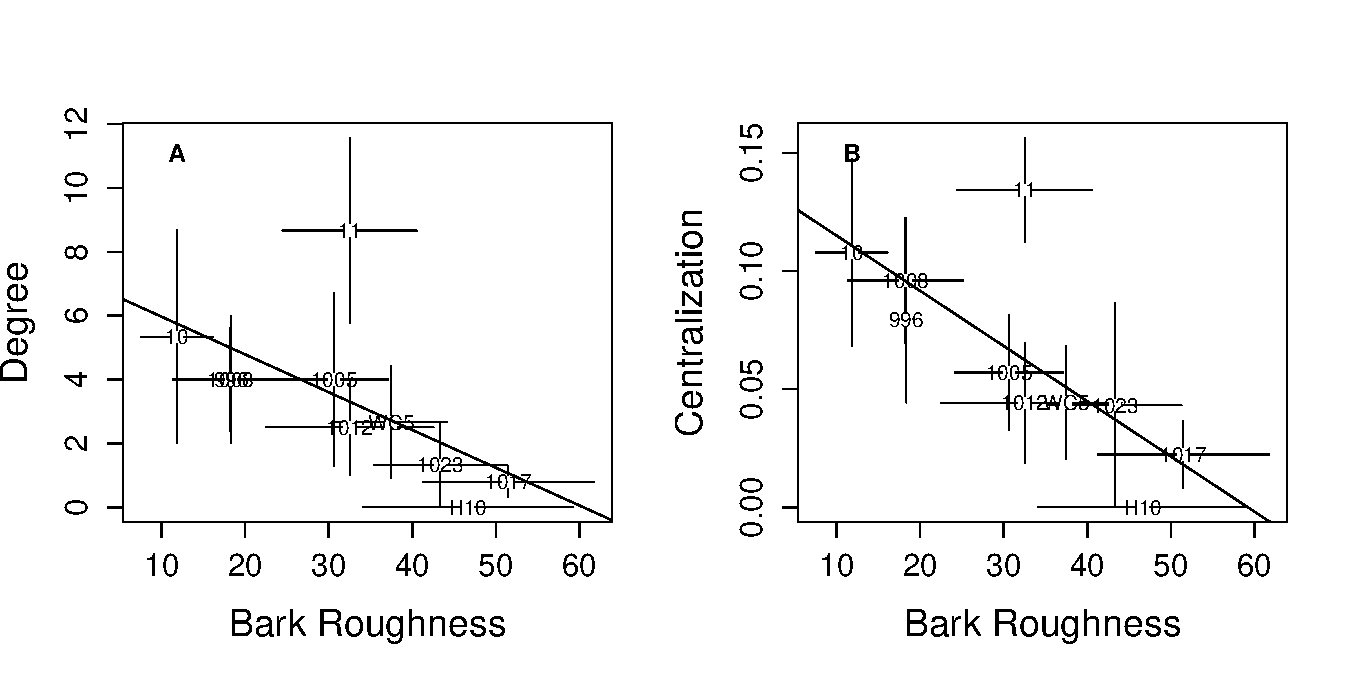
\includegraphics[width=\linewidth]{figures/br_net.pdf}
\caption{Bivariate plots of the negative relationship between bark
  roughness and two network metrics: A) degree and B)
  centralization. Each plot displays the genotype mean ($\pm$ 1 S.E)
  for both variables and a least-squares regression line calculated
  using the genotype means. Generally, as roughness increased the
  number of interactions (degree) and dominance of
  those interactions (centralization) decreased.}
\label{fig:br_net}
\end{figure*}


\section*{Discussion}


\subsection*{Evolutionary Importance of Ecological Network Heritability}

The demonstration of evolution by natural selection requires three key
elements \citep{Conner2004ATextbook}, which multilevel selection
theory posits can occur simultaneously at multiple levels of
ecological organization \citep{Whitham2003,
  Whitham2020IntraspecificEvolution}. First, there must be variation,
which at the community level means variation in species abundance,
richness, interactions and/or interaction network structure. Second,
these differences must be genetically based and heritable in which
community structure is passed from one generation to the next. For
example, numerous studies show that related individuals tend to
support the same communities of insects and microbes, and ecosystem
processes of biodiversity, nutrient cycling and stability, whereas
unrelated individuals support more different communities and ecosystem
processes, per the genetic similarity rule \citep{Bangert2006,
  Bangert2008a, Barbour2009c,
  Whitham2020IntraspecificEvolution}. Third, selection must favor some
communities over other. Given these conditions, selection will lead to
community level change over time (i.e., community evolution). This is
consistent with holobiont theory and empirical studies
\citep{Zilber-Rosenberg2008, Gilbert2012} in which the holobiome
(usually a multicelluar host and its symbionts) is the primary unit of
selection \citep{Bordenstein2015, Johnson2021}.

There are two important functional ramifications of genetically based
variation in network structure. First, and most notably, the current
study shows that the structure of lichen networks on individual trees
is heritable, which is key for selection to act. Heritability (i.e.,
genetic determination) means that there is structure in the spatial or
temporal variation that is created by individuals of foundation
species whose traits are in part determined by underlying trait
differences. Although this variation is inherently a function of both
genetic and environmental effects \citep{Conner2004ATextbook}, the
community and network-level effects are also a function of the scale
of the interaction \citep{Shuster2006COMMUNITYSTRUCTURE-fix,
  Lau2017a}. Second, heritability of network structure suggests that
some amount of interaction network complexity is determined and
therefore could be predicted by genetic identity. Thus, variation in
foundation species traits in space and time create variation in
ecological networks that influences evolutionary dynamics via shifts
in ecological dynamics, such as population demographics and
interactions \citep{Guimaraes2020afix}.

An important implication of this latter point is that intraspecific
variation in a foundation species inherently creates variation in
network structure, whether or not there are feedbacks from the
foundation species to the associated organisms, as suggested
previously by \cite{Lau2016afix}. Thus, the differential survival and
performance of individual tree genotypes will simultaneously result in
selection occurring on the lichen community and network structure that
it supports. Although previous studies have examined aspects of
ecological networks, such as trophic complexity
\citep{Barbour2016GeneticComplexity} and forest stand level
interaction network structure \citep{Lau2016afix,
  Keith2017}, this is the first study that we are aware of to examine
the heritability of network structure with replicated networks at the
genotype scale. Previous work in the evolution of ecological networks
have primarily focused on macro-evolutionary dynamics
\citep{Rezende2007, Weber2017EvolutionMacroevolution,
  Valverde2018TheSpandrel, Harmon2019DetectingInteractions} or have
been simulation based individual-level models that integrate
intraspecific variation to the species level
\citep{Maliet2020AnNetworks}, even though recent syntheses have
pointed to the importance of processes operating across scales of
organization \citep{Guimaraes2020afix}.


\subsection*{Network Structure and Scaling}

Our study demonstrates that the localized environmental differences
determined by the genetic variation within a single tree species can
not only impact community composition, as repeatedly demonstrated in
other community genetics studies \citep{Whitham2006a,
  DesRoches2018TheVariation}, but it can also shape the network of
interactions among community members. Some network structures are
likely to be more stable, either in response to disturbance or via
self-organized dynamics. For example, centralized networks, although
more efficient, are theorized to be more susceptible to targeted
``attacks'' in the terminology of defense networks. As mentioned
previously, one class of networks that are theorized to have
amplifying effects on networks have centralized "star" shapes with one
or a few species at the center and radiating interactions out from the
central core \citep{Lieberman2005EvolutionaryGraphs}. This is
structurally what we have observed with the networks that tend to
occur on some of the genotypes in our study, i.e., the more
centralized networks. It is likely that these networks could function
as hot-spots of evolutionary dynamics resulting from the amplifying
effect of the centralized network structure found on that tree
genotype, as multiple studies have found significant impacts of the
removal of foundation species in different systems \citep{Keith2017,
  DesRoches2018TheVariation}.

Game theoretic applications to ecological networks provide a
theoretical basis that relates to the heritability of network
centralization found in the present study. Although developed at the
population scale, this theory could be applied at the community scale
as well \citep{Lieberman2005EvolutionaryGraphs}. One seemingly useful
direction is the classification of networks into two general
categories, rooted and cyclic, in which rooted networks have
interactions in which evolutionary effects emanate from one or
multiple origins but these effects do not have feedbacks to the
origin, whereas cyclic networks contain feedbacks to one or more
origins. This is equivalent to ``unidirectional'' and ``reciprocal''
genetic effects in the context of IIGE theory
\citep{Whitham2020IntraspecificEvolution}. As we do not have an
estimate of the effect of the lichen at the larger scale of the
fitness of the tree they occur on, we can not determine whether the
lichen networks in this system are cyclic or not. In terrestrial
ecosystems, lichens play important ecological roles, such as substrate
stabilization \citep{Root2011BioticWashington} and nitrogen fixation
\citep{Nelson2018LichenHelens}. Some epiphytic lichens can have
demonstrable effects on the availability of nutrients for the trees
that are associated with \citep{Norby1989NitrogenDioxide}.  Although
none of the lichens the present study's system is known to fix
nitrogen, it is possible that they might add micro-nutrients or
provide some other unobserved benefit to their host trees.

Elucidating the presence of and quantifying such feedbacks would
permit the determination of the cyclic nature evolutionary
dynamics. If there are positive effects of lichens on host trees that
might increase their ability to respond to environmental stress, then
selection could enhance tree performance and trees with superior
communities are more likely to survive.  \cite{Gehring2014PlantChange,
  Gehring2017afix} showed this with ectomycorrhizal communities in which
trees with superior mutualist communities were more likely to survive
drought and community evolution occurred
\citep{Whitham2020IntraspecificEvolution}.  However, such feedbacks to
the higher level of the foundation species are not a requirement for
evolution, and, regardless of whether networks are rooted (no
feedbacks) or cyclic (feedbacks present), selection at the community
level leading to evolution can still occur.  Specifically within the
context of the current study, even if lichens and their interactions
do not feed back to affect the performance and ultimate fitness of the
tree on which they reside, non-random death of trees, such as those
observed for drought in arid systems \cite{Sthultz2009, Gehring2017afix},
can still result in selection at the community level and
evolution. For example, when a tree dies from some event (e.g., a
drought, fire, storm, etc.), its lichen network is selected against
while intact networks persist on other trees that survive this
selection event.

The importance of the scale of network organization to create
hierarchical structure \citep{Guimaraes2020afix} and the
potential for foundation species to create this structure in the vast
majority of ecosystems \citep{Ellison2005, Whitham2006a} suggests that
future work would be aided by determining species with large
differences in body-size and longevity. Such differences are likely
contributing to interaction network structure (e.g., modules and
centralized species). Many ecological network studies that have an
evolutionary context have focused on asymmetry (e.g., nestedness) and
the quantification of its structure in communities
\citep{Bascompte2006, Diaz-Castelazo2010, Guimaraes2011,
  Thompson2013}. Although there is growing evidence that the
nestedness of mutualistic networks is not necessarily the result of
selection for systems-level properties but could be either the
numerical result of asymptotic abundance distributions leading to
uneven interaction frequencies \citep{Staniczenko2013TheNetworks}
and/or a by-product of selection and divergence creating network
``spandrels'' in ecosystems \citep{Valverde2018TheSpandrel}, the
findings of these studies have generally supported the hypothesis that
nestedness (the degree to which species tend to interact with similar
subsets of the community) tends to promote stability in mutualistic,
primarily bipartite (i.e., two-mode), networks and that modularity
contributes to the stabilization of antagonistic networks
\citep{Elias2013EvolutionaryNetwork,
  Grilli2016afix}. We were not able to examine
nestedness or modularity of the lichen networks in the current study,
as metrics for analyzing weighted, directed \textit{and} signed
networks could not be found. Future network theoretic developments
will hopefully produce the appropriate metrics to conduct these
analyses.

\subsection*{Community Composition and Quantifying Network Structure}

Our findings point to the importance of quantifying interactions and
not simply using community composition as a proxy. We did not observe
compositional differences using the same data from which the lichen
networks were derived. Thus, if we only had analyzed the composition
data, we would have concluded no response of the lichen community to
tree genotype, even though the interactions among lichen species vary
among genotypes. Community composition of lichens has previously been
observed to be different among tree genotypes in the same experimental
garden \citep{Lamit2011, Lamit2015a}. The different results observed
in the present study is likely a result of differences in lichen
quantification and the tree genotypes observed leading to overall
higher abundances of observed lichens to assure the possibility of
observing lichen interactions. Thus, the findings of the current study
do not negate the previous study, as the quantification methods were
different for community composition, but they do support the
conclusion that composition is not a proxy for interactions in complex
communities.

This is a concern, as such differences in network structure could
occur without observable differences in species richness or community
composition, which has been the primary focus of the majority of
community genetics studies
\citep{Whitham2020IntraspecificEvolution}. It is possible that these
underlying differences in interactions among lichens could lead to
differences in community composition at a future point in time via
their effects on species abundances
\citep{Shuster2006COMMUNITYSTRUCTURE-fix}; however, this is not needed
for evolutionary dynamics to occur via selection that produces shifts
in trait distributions without shifting species abundance
distributions, which is possible under stabilizing, disruptive and
directional selection \citep{Conner2004ATextbook}. Thus, it is
imperative that further community genetics research assess or at least
be aware of the potential effects of variation in interactions and not
just observe species abundances, otherwise community level genetic
effects may be underestimated, especially when cumulative interaction
effects are taken into account
\citep{Borrett2007FunctionalProliferation, Borrett2010}. Furthermore,
the demonstration of the heritability of interaction networks, without
significant differences in community composition, provides clear
empirical evidence that IIGEs need to encompass the structure of
interaction networks.

Although IIGE theory provides a quantitative framework within which to
approach evolutionary theory at higher levels of biological
organization (from populations to communities and ecosystems), this
theory has focused on modeling the strong effects of foundation
species \citep{Shuster2006COMMUNITYSTRUCTURE-fix, Whitham2012afix,
  Whitham2020IntraspecificEvolution} and has not yet integrated
developments from the ecological or evolutionary network theory
literature. Thus, it has not developed a way to examine complex
interactions among species; however, previous studies have
demonstrated this network context is likely to be important, as
altering the structure of interaction networks provides a means for
genetic effects to be dampened or magnified within the system of
interacting species \citep{Smith2011, Keith2017}. Such a synthesis
necessitates a much greater effort than can be afforded in this paper.
However, we recommend continued focus on foundation species, which are
by definition ``central'' within the system of interactions and their
direct and indirect effects should generally be greater than other
species \citep{Ellison2005}. Thus, when the more centralized
(foundation) species have genetically based interactions, genetic
effects will tend to be propagated and possibly magnified in the
community. Identifying central species the modules of species that
they interact with provides a promising in-road to understanding
ecological complexity, as the presence of asymmetries in ecosystems,
such as hierarchy created by foundation species via differences in
body size and/or life-history strategies, tend to create
directionality in both ecological and evolutionary dynamics
\citep{Ellison2005, Bascompte2006, Whitham2020IntraspecificEvolution,
  Guimaraes2020afix}.



\subsection*{Conclusion}

We found support for both of our hypotheses. First, tree genotype
influenced the network structure of lichen communities associated with
narrowleaf cottonwoods in a riparian forest ecosystem. Network
similarity and metrics of network structure tended to be more similar
on trees of the same genotype. Second, the genetically based trait,
bark roughness, was observed to affect network variation, largely via
shifts in positive in-coming and out-going interactions. Although bark
roughness has been shown previously to be an important tree trait
influencing bark lichens \citep{Lamit2015a}, this is the first
demonstration of a link from plant genetics to lichen network
structure via this trait. As heritable variation is the raw material
for natural selection to act upon, a genetic basis for interaction
network structure indicates that conserving genetic variation is
important to consider in efforts to restore or preserve complex
species interactions and their associated ecosystem functions \citep{
  Whitham2012afix, Evans2013, Barraclough2015,
  Whitham2020IntraspecificEvolution}. Network modeling and analysis
will provide useful tools for the identification of species within
network modules that are most important to study in systems where
little is known about the natural history of organisms in an
ecosystem. Collectively, such investigations will bring us closer to
understanding the evolutionary drivers of Darwin's entangled bank and
the interconnectedness of species in complex communities
\citep{Darwin1859, Dattilo2016fix}.



\subsection*{Acknowledgments}

This work was supported by National Science Foundation grants
DEB-0425908 and DEB-1340852, the NSF funded Northern Arizona
University Genes to Ecosystems Integrative Graduate Research
Traineeship (IGERT) and the ARCS Foundation (Phoenix Chapter). Thanks
also to the Ogden Nature Center staff who helped to maintain the
common garden experiments and Drs. Todd Wojtowicz, Luke Evans and
David Solance Smith for assistance with lichen network observations.

%% \subsection*{Figures and Tables}

%% Use the table and tabular commands for basic tables --- see
%% Table~\ref{tab:widgets}, for example. You can upload a figure
%% (JPEG, PNG or PDF) using the project menu. To include it in your
%% document, use the includegraphics command as in the code for
%% Figure~\ref{figures/fig:view} below.

%% \begin{figure}[ht]
%% \centering
%% \includegraphics[width=0.7\linewidth]{figures/frog}
%% \caption{An example image of a frog.}
%% \label{fig:view}
%% \end{figure}

%% \begin{table}[ht]
%% \centering
%% \begin{tabular}{l|r}
%% Item & Quantity \\\hline
%% Candles & 4 \\
%% Fork handles & ?  
%% \end{tabular}
%% \caption{\label{tab:widgets}An example table.}
%% \end{table}


%% \bibliography{lichen_network_genetics,manual,fixed,r_pkgs}
\bibliography{bibliography}

\end{document}
